\chapter{Lab 4 - Controlled Sources}

%%%%%%%%%%%%%%%%%%%%%%%%%%%%%%%%%%%%%%%%%%%%%%%%%%%%%%%%%%%%%%%%%%%%%%%%%%%%%%%%%%%%%%%%%%%%%%%%%%%%%%%
\section{Objective}
%%%%%%%%%%%%%%%%%%%%%%%%%%%%%%%%%%%%%%%%%%%%%%%%%%%%%%%%%%%%%%%%%%%%%%%%%%%%%%%%%%%%%%%%%%%%%%%%%%%%%%%

The purpose of this lab is gain an understanding of controlled voltage sources and the effects of input resistance, output resistance, and feedback. 

%%%%%%%%%%%%%%%%%%%%%%%%%%%%%%%%%%%%%%%%%%%%%%%%%%%%%%%%%%%%%%%%%%%%%%%%%%%%%%%%%%%%%%%%%%%%%%%%%%%%%%%
\section{Materials}
%%%%%%%%%%%%%%%%%%%%%%%%%%%%%%%%%%%%%%%%%%%%%%%%%%%%%%%%%%%%%%%%%%%%%%%%%%%%%%%%%%%%%%%%%%%%%%%%%%%%%%%

\begin{itemize}
	\item Laptop with LTSpice
\end{itemize}

%%%%%%%%%%%%%%%%%%%%%%%%%%%%%%%%%%%%%%%%%%%%%%%%%%%%%%%%%%%%%%%%%%%%%%%%%%%%%%%%%%%%%%%%%%%%%%%%%%%%%%%
\section{Introduction}
%%%%%%%%%%%%%%%%%%%%%%%%%%%%%%%%%%%%%%%%%%%%%%%%%%%%%%%%%%%%%%%%%%%%%%%%%%%%%%%%%%%%%%%%%%%%%%%%%%%%%%%

A controlled source references a voltage or current and in turn generates a voltage or current, often amplifying the reference in the process. Four possible variations exist: 
	\begin{itemize}
		\item Voltage Controlled Voltage Source (VCVS)
		\item Voltage Controlled Current Source (VCCS)
		\item Current Controlled Voltage Source (CCVS)
		\item Current Controlled Current Source (CCCS)
	\end{itemize}
\noindent For this course, the primary concern is a VCVS because is serves as part of the model for an amplifier. 

\subsection{Voltage Controlled Voltage Source}

As the name implies, a VCVS generates a voltage controlled by a different voltage. Usually this voltage is across a resistance but for the ideal case, the resistance is infinite and appears as an open circuit. Similarly, the output is simply the gain, $A$, multiplied by the control voltage, $V_i$, when the output resistance is zero and appears as a wire. Consider the models for a VCVS show in \hyperref[fig:4sourcemodel]{Figure \ref*{fig:4sourcemodel} (a) through (c)}. For the ideal case, (a) and (b), the voltage drop $V_i$ provides the control voltage for the controlled source which generates a voltage output of $A V_i$. Practically, the input and output resistances must be considered as shown in (c). 

\begin{figure} [h]
	\centering
		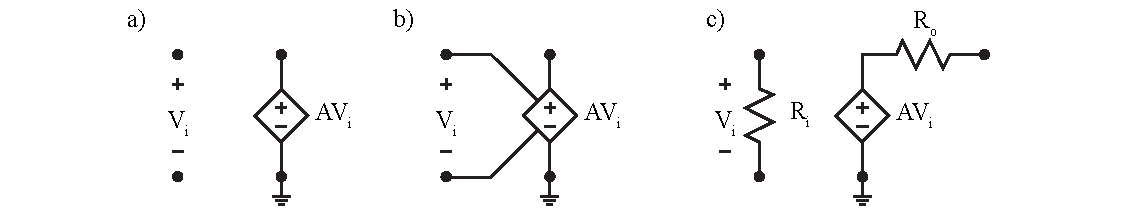
\includegraphics[width=1\textwidth]{Lab4AidealSource.pdf}
	\caption{Representations of a voltage controlled voltage source, ideal model (a), variation used in LTspice (b), and a model with an input and output resistance (c).} \label{fig:4sourcemodel}
\end{figure}


%%%%%%%%%%%%%%%%%%%%%%%%%%%%%%%%%%%%%%%%%%%%%%%%%%%%%%%%%%%%%%%%%%%%%%%%%%%%%%%%%%%%%%%%%%%%%%%%%%%%%%%%
%\subsection{Input and Output Resistance}
%%%%%%%%%%%%%%%%%%%%%%%%%%%%%%%%%%%%%%%%%%%%%%%%%%%%%%%%%%%%%%%%%%%%%%%%%%%%%%%%%%%%%%%%%%%%%%%%%%%%%%%%


%%%%%%%%%%%%%%%%%%%%%%%%%%%%%%%%%%%%%%%%%%%%%%%%%%%%%%%%%%%%%%%%%%%%%%%%%%%%%%%%%%%%%%%%%%%%%%%%%%%%%%%
\subsection{Feedback}
%%%%%%%%%%%%%%%%%%%%%%%%%%%%%%%%%%%%%%%%%%%%%%%%%%%%%%%%%%%%%%%%%%%%%%%%%%%%%%%%%%%%%%%%%%%%%%%%%%%%%%%

%Obviously the gain of the controlled source is the variable most affected by the Monte Carlo simulations but that's expected, the output voltage depends directly on the input voltage multiplied by the gain of the controlled source. While this is not a serious problem for a small gain, 10, it is a serious problem when the gain is large, on the order of $10^5$. 

%Before the advent of modern electronics with better control of the fabrication process, the gain would often vary over a wide range which proved problematic when an exact gain was desired. While convenient to set the model gain of the controlled source to a value of 10, it's not practical, the gain can't be changed after production when a gain of 15 or 1 is desired. Often a large gain would be used in order to amplify small signals but this presents another problem, the input must be small in order to prevent the output from clipping or saturation, beyond the scope of our current mode. The answer to these two problems, high variation in the gain and high gain, is feedback. Feeding back the output signal back to the input allows the overall output to be dependent on external components, resistors, that can be well controlled.

The combination of an amplifier with feedback can be represented many ways. One of the generic ways is a signal flow diagram as shown in \hyperref[fig:4sigflow]{Figure \ref*{fig:4sigflow}}. 

\begin{figure} [h]
	\centering
		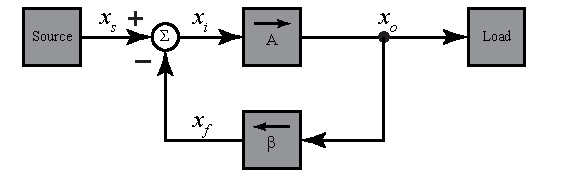
\includegraphics[width=0.5\textwidth]{Lab4signalflow.pdf}
	\caption{A signal flow diagram for an amplifier with feedback. Each voltage is represented by some value $x$, with an amplifier of gain A, and a feedback factor of $\beta$.} \label{fig:4sigflow}
\end{figure}

The amplifier has a gain, A, which is called the open-loop gain and represents the gain from the input, $x_i$, of the amplifier to the output, $x_o$. This is described by the equation

\begin{equation}
	x_o = A x_i
\end{equation}

\noindent In this example, the output is feedback through a feedback network with a feedback factor, $\beta$. Which gives the feedback voltage, $x_f$, equal to the output voltage, $x_o$, times the feedback factor, $\beta$.

\begin{equation}
	x_f = \beta x_o
\end{equation}

\noindent The feedback voltage, $x_f$, is then subtracted from the source signal, $x_s$, which gives the input to the amplifier, $x_i$. 

\begin{equation}
	x_i = x_s - x_f
\end{equation}

\noindent Here it's important to recognize that the loading effects of the load and source have been neglected as this is a generic case with finite gain. The total gain of the system, with feedback, then becomes

\begin{equation}
	A_f \equiv \frac{x_o}{x_s} = \frac{A}{1 + A \beta}
\end{equation}

\noindent This equation represents the closed loop gain of the system which is smaller than the open loop gain by a factor of $1+A\beta$, called the amount of feedback. The quantity A$\beta$ is the loop gain and must be positive. Often the loop gain is large, $A\beta \gg 1$, or simply A is large, which simplifies the closed loop gain to

\begin{equation}
	A_f \simeq \frac{1}{\beta}
\end{equation}

\noindent Which gives a result entirely dependent on the feedback factor. This is an important because if the gain, A, is large, the closed loop gain will depend entirely on elements in the feedback network. 

%%%%%%%%%%%%%%%%%%%%%%%%%%%%%%%%%%%%%%%%%%%%%%%%%%%%%%%%%%%%%%%%%%%%%%%%%%%%%%%%%%%%%%%%%%%%%%%%%%%%%%%
\section{Pre-Lab Requirements}
%%%%%%%%%%%%%%%%%%%%%%%%%%%%%%%%%%%%%%%%%%%%%%%%%%%%%%%%%%%%%%%%%%%%%%%%%%%%%%%%%%%%%%%%%%%%%%%%%%%%%%%

Complete the following using LTspice.

%%%%%%%%%%%%%%%%%%%%%%%%%%%%%%%%%%%%%%%%%%%%%%%%%%%%%%%%%%%%%%%%%%%%%%%%%%%%%%%%%%%%%%%%%%%%%%%%%%%%%%%
\subsection{Simulating a Controlled Source} \label{ssec:4simcs}
%%%%%%%%%%%%%%%%%%%%%%%%%%%%%%%%%%%%%%%%%%%%%%%%%%%%%%%%%%%%%%%%%%%%%%%%%%%%%%%%%%%%%%%%%%%%%%%%%%%%%%%

\begin{figure} [h]
	\centering
		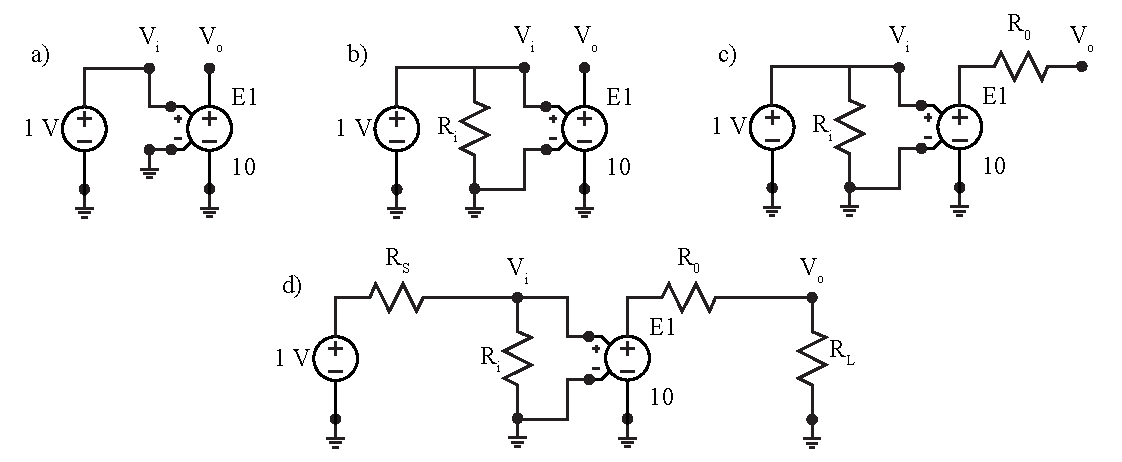
\includegraphics[width=1\textwidth]{Lab4ALTsource.pdf}
	\caption{Different configurations for a VCVS in LTspice: the ideal case (a), with an input resistance (b), with an input resistance and output resistance (c), and with a source and load resistance (d).} \label{fig:4sourcespice}
\end{figure}


\begin{enumerate}
	\item Setup a simple voltage controlled voltage source in LTspice with a gain of 10 as shown in \hyperref[fig:4sourcespice]{Figure \ref*{fig:4sourcespice} (a)}. Use the e component in LTspice, voltage dependent voltage source, and set the gain, E, to 10 and run a DC operating point solution to confirm that the output of the controlled source is 10 V. Table the input, $V_i$, and output, $V_o$, voltages. \label{itm:4ssec1itm1}
	\item Connect an input resistance from the voltage input to ground as shown in \hyperref[fig:4sourcespice]{Figure \ref*{fig:4sourcespice} (b)}. Set the resistance to 10 k$\Omega$ and re-run the DC operating point simulation, table the values for $V_i$ and $V_o$.
	\item Connect an output resistance form the controlled source output as shown in \hyperref[fig:4sourcespice]{Figure \ref*{fig:4sourcespice} (c)}. Set the resistance to 10 k$\Omega$ and re-run the DC operating point simulation, table the values for $V_i$ and $V_o$.
	\item Connect the circuit as shown in \hyperref[fig:4sourcespice]{Figure \ref*{fig:4sourcespice} (d)} with a source, $R_S$, and load, $R_L$, resistance. Set both values to 50 $\Omega$ and re-run the DC operating point simulation, table the values for $V_i$ and $V_o$. \label{itm:4ssec1itm4}
	\item Step through different values of $R_i$ from 0.1 to 1Meg in powers of 10 and determine the best value for the input resistance. Plot the input voltage, $V_i$, on a log scale and save an image of the plot and circuit. \label{itm:4ssec1itm5}
	\item Using the value of $R_i$ from the previous step, step through different values of $R_o$ from 0.1 to 1Meg in powers of 10 and determine the best value for the output resistance. Plot the output voltage, $V_o$, on a log scale and save an image of the plot and circuit. \label{itm:4ssec1itm6}
\end{enumerate}

%%%%%%%%%%%%%%%%%%%%%%%%%%%%%%%%%%%%%%%%%%%%%%%%%%%%%%%%%%%%%%%%%%%%%%%%%%%%%%%%%%%%%%%%%%%%%%%%%%%%%%%
\subsection{Monte Carlo Simulations} \label{ssec:4MonteCarlo}
%%%%%%%%%%%%%%%%%%%%%%%%%%%%%%%%%%%%%%%%%%%%%%%%%%%%%%%%%%%%%%%%%%%%%%%%%%%%%%%%%%%%%%%%%%%%%%%%%%%%%%%

\begin{figure} [h]
	\centering
		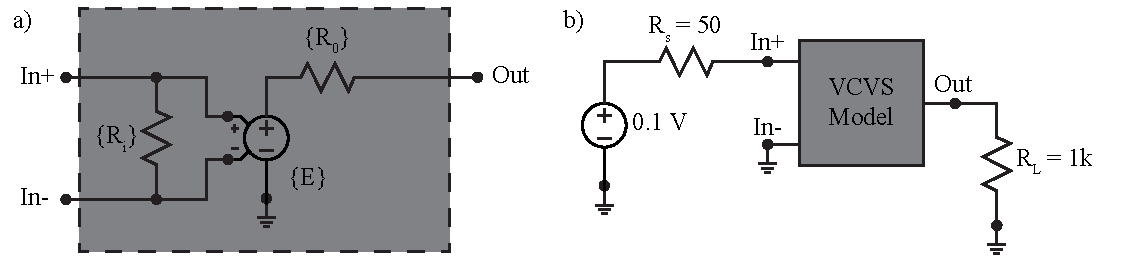
\includegraphics[width=1\textwidth]{Lab4Agenmodel.pdf}
	\caption{A general model for a voltage controlled voltage source with input and output resistance (a) and model used in conjunction with a DC source and a source and load resistance (b). Note that each of the values for the two resistors and the gain are LTspice variables, denoted by the curly brackets, \{\}.} \label{fig:4genmod}
\end{figure}

\begin{enumerate}
	\item Create a sub-circuit of the VCVS from \hyperref[ssec:4simcs]{Subsection \ref*{ssec:4simcs}} as shown in \hyperref[fig:4genmod]{Figure \ref*{fig:4genmod} (a)}. Set the input resistance and output resistance to the previously determined values and the gain to 10. The second half of this video, \url{http://www.linear.com/solutions/7723}, is a helpful tutorial for creating a sub-circuit (symbol) from an already created circuit. Note that default parameters are defined in the subcircuit. To quickly make a subcircuit, in LTspice navigate to the Hierarchy tab, and select "Open this sheet's symbol". This will prompt you to generate a new symbol file, select yes. You can now access this symbol file under the component selection option. All you need to do is change the top directory (the drop down list at the top of the page). Your top directory will be wherever on your computer you created your original LTspice .asc file, and the symbol file will have been generated and must remain in that same directory/folder.
	\item Connect a 0.1V DC voltage source in series with a source resistance of 50 $\Omega$ to the positive input terminal, connect the negative input terminal to ground, and a 1k $\Omega$ resistor to ground at the output as shown in \hyperref[fig:4genmod]{Figure \ref*{fig:4genmod} (b)}.
	\item Run a Monte Carlo simulation for the gain, E, of the VCVS. Set the tolerance to 0.1 (10\%) and run the simulation for 1000 iterations. The Monte Carlo function call can be passed in as a variable to the VCVS model where E = \{mc\{10,tol\}\} in the Value field for the Value attribute. Plot the output voltage and save an image of the circuit and plot. \label{itm:4ssec2itm3}
	\item Repeat the Monte Carlo simulation for the input resistance, Ri. Save an image of the output voltage plot. \label{itm:4ssec2itm4}
	\item Repeat the Monte Carlo simulation for the output resistance, Ro. Save an image of the output voltage plot. \label{itm:4ssec2itm5}
\end{enumerate}

%%%%%%%%%%%%%%%%%%%%%%%%%%%%%%%%%%%%%%%%%%%%%%%%%%%%%%%%%%%%%%%%%%%%%%%%%%%%%%%%%%%%%%%%%%%%%%%%%%%%%%%
\subsection{Feedback} \label{ssec:4Feedback}
%%%%%%%%%%%%%%%%%%%%%%%%%%%%%%%%%%%%%%%%%%%%%%%%%%%%%%%%%%%%%%%%%%%%%%%%%%%%%%%%%%%%%%%%%%%%%%%%%%%%%%%

The VCVS model developed in previous sections has been re-drawn using the more common symbol for an amplifier as shown in \hyperref[fig:4feedbackcombo]{Figure \ref*{fig:4feedbackcombo} (a)}. However, the model is still the same and it's not required to redraw your model. 

\begin{figure} [h]
	\centering
		\includegraphics[width=1\textwidth]{Lab4AvcvsTri.pdf}
	\caption{The VSCS model redrawn as the more common amplifier model symbol (a), unity gain configuration (b), and non-inverting gain configuration (c).} \label{fig:4feedbackcombo}
\end{figure}

\begin{enumerate}
	\item Construct the circuit as shown in \hyperref[fig:4feedbackcombo]{Figure \ref*{fig:4feedbackcombo} (b)}. The resistors $R_S$ and $R_L$ remain 50 $\Omega$ and 1 k$\Omega$ respectively. 
	%\item Calculate the ideal gain, with and without finite gain, for this circuit, \hyperref[fig:4feedbackcombo]{Figure \ref*{fig:4feedbackcombo} (b)}. Assume the input resistance is infinite, the gain is infinite and finite, $10\times10^5$, and the output resistance is zero. \label{itm:4ssec3itm2}
	\item Run a Monte Carlo simulation for the gain, E, of the VSVS model. Set the gain to 10E5, tolerance to 0.3 (30\%), and run the simulation for 1000 iterations. Plot the output voltage and save an image of the circuit and plot. \label{itm:4ssec3itm3}
	\item Construct the circuit as shown in \hyperref[fig:4feedbackcombo]{Figure \ref*{fig:4feedbackcombo} (c)}. Set $R_2$ to 2 k$\Omega$ and $R_1$ to 1 k$\Omega$. The resistors $R_S$ and $R_L$ remain 50 $\Omega$ and 1 k$\Omega$ respectively. 
	%\item Calculate the ideal gain, with and without finite gain, for this circuit, \hyperref[fig:4feedbackcombo]{Figure \ref*{fig:4feedbackcombo} (c)}. Assume the input resistance is infinite, the gain is infinite and finite, $10\times10^5$, and the output resistance is zero. \label{itm:4ssec3itm5}
	\item Run a Monte Carlo simulation for the gain, E, of the VSVS model. Set the gain to 10E5, tolerance to 0.3 (30\%), and run the simulation for 1000 iterations. Plot the output voltage and save an image of the circuit and plot. \label{itm:4ssec3itm6}
\end{enumerate} 

%%%%%%%%%%%%%%%%%%%%%%%%%%%%%%%%%%%%%%%%%%%%%%%%%%%%%%%%%%%%%%%%%%%%%%%%%%%%%%%%%%%%%%%%%%%%%%%%%%%%%%%
\section{In-Lab Requirements}
%%%%%%%%%%%%%%%%%%%%%%%%%%%%%%%%%%%%%%%%%%%%%%%%%%%%%%%%%%%%%%%%%%%%%%%%%%%%%%%%%%%%%%%%%%%%%%%%%%%%%%%

The following must be completed and submitted to Canvas before the start of lab. 

\begin{enumerate}
	\item \hyperref[ssec:4simcs]{Subsection \ref*{ssec:4simcs}}:
		\begin{enumerate}
			\item Items \hyperref[itm:4ssec1itm1]{\ref*{itm:4ssec1itm1}} - \hyperref[itm:4ssec1itm1]{\ref*{itm:4ssec1itm4}}: Table of input and output voltages. 
			\item \hyperref[itm:4ssec1itm5]{Item \ref*{itm:4ssec1itm5}}: Image of circuit and plot of the input voltage.
			\item \hyperref[itm:4ssec1itm6]{Item \ref*{itm:4ssec1itm6}}: Image of circuit and plot of the output voltage.
		\end{enumerate}
	\item \hyperref[{ssec:4MonteCarlo}]{Subsection \ref*{ssec:4MonteCarlo}}:
		\begin{enumerate}
			\item \hyperref[itm:4ssec2itm3]{Item \ref*{itm:4ssec2itm3}}: Image of circuit and plot of the output voltage.
			\item \hyperref[itm:4ssec2itm4]{Item \ref*{itm:4ssec2itm4}}: Plot of the output voltage.
			\item \hyperref[itm:4ssec2itm5]{Item \ref*{itm:4ssec2itm5}}: Plot of the output voltage.
		\end{enumerate}
	\item \hyperref[ssec:4Feedback]{Subsection \ref*{ssec:4Feedback}}:
		\begin{enumerate}
			%\item \hyperref[itm:4ssec3itm2]{Item \ref*{itm:4ssec3itm2}}: Ideal gain.
			\item \hyperref[itm:4ssec3itm3]{Item \ref*{itm:4ssec3itm3}}: Image of circuit and plot of the output voltage.
			%\item \hyperref[itm:4ssec3itm5]{Item \ref*{itm:4ssec3itm5}}: Ideal gain. 
			\item \hyperref[itm:4ssec3itm6]{Item \ref*{itm:4ssec3itm6}}: Image of circuit and plot of the output voltage.
		\end{enumerate}
\end{enumerate}

Complete the following items in lab.

%%%%%%%%%%%%%%%%%%%%%%%%%%%%%%%%%%%%%%%%%%%%%%%%%%%%%%%%%%%%%%%%%%%%%%%%%%%%%%%%%%%%%%%%%%%%%%%%%%%%%%%
\subsection{Worst Case Analysis} \label{ssec:4worstcase}
%%%%%%%%%%%%%%%%%%%%%%%%%%%%%%%%%%%%%%%%%%%%%%%%%%%%%%%%%%%%%%%%%%%%%%%%%%%%%%%%%%%%%%%%%%%%%%%%%%%%%%%

While Monte Carlo analysis is useful for looking at a range of possible values, often times it's important to see the potential worst case values given a specified tolerance. Use the VCVS model that was previusly devloped with the values of $R_i$ and $R_o$ previously defined and a gain of 10E5. 

\begin{figure} [h]
	\centering
		\includegraphics[width=1\textwidth]{Lab4wc.pdf}
	\caption{Non-inverting configuration with the necessary resistor values for a worst case simulation (a) and inverting configuration with the necessary resistor values for a worst case simulation (b).} \label{fig:4wcckts}
\end{figure}


\begin{enumerate}
	\item Construct the circuit as shown in \hyperref[fig:4wcckts]{Figure \ref*{fig:4wcckts} (a)}
	\item Run a DC operating point simulation with the following additional parameters:
\begingroup
    \fontsize{10pt}{12pt}\selectfont
	\begin{verbatim}
		.func binary(run,index) floor(run/(2**index))-2*floor(run/(2**(index+1)))
		.func wc(nom,tol,index) if(run==numruns,nom,if(binary(run,index),nom*(1+tol),nom*(1-tol)))
		.param numruns=4
		.step param run 0 4 1
		.param tol=0.05
	\end{verbatim}
\endgroup

	\item Plot the output voltage and save an image of the plot. Determine the worst case results, which resistor tolerances, that gives the highest and lowest output voltages. \label{itm:4ssec4itm3}
	\item Repeat the simulation for a tolerance of 0.01 (1\%), 0.005 (0.5\%), 0.001 (0.1\%), 0.0005 (0.05\%), and 0.0001 (0.01\%). For each case, table the high, low output voltages, and determine the cost of the components. Use the following Digikey link to determine pricing: \url{http://digikey.com}. Search through hole resistors, select the ones in-stock for 0.25 Watt, Carbon Film according to the required tolerance.  \label{itm:4ssec4itm4}
	\item Construct the circuit as shown in \hyperref[fig:4wcckts]{Figure \ref*{fig:4wcckts} (b)}
	\item Run a DC operating point simulation with the parameters previously stated.
	\item Plot the output voltage and save an image of the plot. Determine the worst case results that gives the highest and lowest output voltages. \label{itm:4ssec4itm7}
	\item Repeat the simulation for a tolerance of 0.01 (1\%), 0.005 (0.5\%), 0.001 (0.1\%), 0.0005 (0.05\%), and 0.0001 (0.01\%). For each case, table the high, low output voltages, and determine the cost of the components. \label{itm:4ssec4itm8}
\end{enumerate}

%%%%%%%%%%%%%%%%%%%%%%%%%%%%%%%%%%%%%%%%%%%%%%%%%%%%%%%%%%%%%%%%%%%%%%%%%%%%%%%%%%%%%%%%%%%%%%%%%%%%%%%
\section{Write Up}
%%%%%%%%%%%%%%%%%%%%%%%%%%%%%%%%%%%%%%%%%%%%%%%%%%%%%%%%%%%%%%%%%%%%%%%%%%%%%%%%%%%%%%%%%%%%%%%%%%%%%%%

Include the following in the write up.

\begin{enumerate}
	\item \hyperref[ssec:4worstcase]{Subsection \ref*{ssec:4worstcase}}
		\begin{enumerate}
			\item \hyperref[itm:4ssec4itm3]{Item \ref*{itm:4ssec4itm3}}: Output voltage plot for a 5\% tolerance and the highest and lowest output voltage cases. 
			\item \hyperref[itm:4ssec4itm4]{Item \ref*{itm:4ssec4itm4}}: Tabled output voltage range and pricing for different resistor tolerances. 
			\item \hyperref[itm:4ssec4itm7]{Item \ref*{itm:4ssec4itm7}}: Output voltage plot for a 5\% tolerance and the highest and lowest output voltage cases. 
			\item \hyperref[itm:4ssec4itm8]{Item \ref*{itm:4ssec4itm8}}: Tabled output voltage range and pricing for different resistor tolerances. 
		\end{enumerate}
\end{enumerate}

Discuss the benefits of feedback, worst case analysis for different resistor tolerances, and the cost/benefit trade off for different resistor tolerances.

For all lab write up submissions and reports the backgrounds for LTSpice and Waveforms should be changed from dark background to light background to make them readable for grading. 

If the prelab simulation is incorrect, do not compare the in lab results to wrong values.  Correct numbers or circuit schematics should be used in the write-up report.

